% Fuentes que no vi:
% https://www.youtube.com/@AuxiRolando

\documentclass[a4paper]{article}
\usepackage[margin=1.5cm]{geometry}

%\documentclass[11pt]{article}
%\usepackage[paperwidth=9cm,paperheight=60cm,margin=0.4cm]{geometry}

\usepackage{multicol}
\usepackage{enumitem}
\usepackage{graphicx}

%Links
\usepackage[colorlinks = true,
            linkcolor = blue,
            urlcolor  = blue,
            citecolor = blue,
            anchorcolor = blue]{hyperref}

%Simbolos matemáticos
\usepackage{amsmath}
\usepackage{amssymb}

%Enumeracion
\usepackage{enumitem}

%Páginas sin numeración
\pagestyle{empty}

%Interlineado
\renewcommand{\baselinestretch}{1.5}

%Arreglar comillas
\usepackage [autostyle]{csquotes}
\MakeOuterQuote{"}

%Macros
\newcommand{\Item}{\item[\stepcounter{enumii}$\blacktriangleright$\textbf{(\alph{enumii})}]} %Negrita en algunos items
\newcommand{\answer}{\item[**]}
\newcommand{\exercise}{\item}

%Logic macros
\newcommand{\then}{\to}
\newcommand{\eq}{\leftrightarrow}
\newcommand{\xor}{\veebar}
\newcommand{\nor}{\downarrow}
\newcommand{\nimply}{\nrightarrow}
\newcommand{\nand}{\uparrow}
\newcommand{\Then}{\Rightarrow}
\newcommand{\Eq}{\Leftrightarrow}


\begin{document}

\noindent \hrulefill 
\vspace{-7pt}
\begin{center} 
	\textbf{ Práctica 1: Lógica proposicional y de primer orden } \\
	Comisión: Rodrigo Cossio-Pérez y Leonardo Lattenero
\end{center}
\vspace{-10pt}
\hrulefill


\begin{enumerate}

	\exercise Reconocer las funciones del lenguaje e indicar qué casos son proposiciones. Si son proposiciones, indicar su valor de verdad.
	\begin{multicols}{2}
	\begin{enumerate} [label=(\alph*)]
		\Item Hoy es martes 
		\answer Función informativa, es proposición. El valor de verdad dependerá del día.

		\item ¿Venís hoy a clase?
		\answer Función interrogativa, no es proposición.

		\Item Vaya a visitar las playas de la costa de Buenos Aires
		\answer Función imperativa, no es proposición.

		\item Fuí a visitar las playas de la costa de Buenos Aires 
		\answer Función informativa, es proposición. El valor de verdad depende de la persona que lo lea.

		\Item ¿Está lloviendo?
		\answer Función interrogativa, no es proposición.

		\Item Me parece que sí 
		\answer Función informativa, es proposición. El valor de verdad no depende de si llueve o no, depende de si quien lo dice le parece que llueve o no. Si el narrador está engañando será falsa, si realmente cree que sí será verdadera.

		\item Tal vez llueve
		\answer Función informativa, es proposición. Podemos indicar si es verdadero en momentos y lugares donde es posible que llueva, mientras que será falsa si en lugares donde no es posible que llueva.

		\item ¡Auch!
		\answer Función exclamativa, no es una proposición. Notar que gritar "Me acabo de lastimar" sí sería es una proposición.

		\Item En las aulas de la UNQ
		\answer No es proposición ya que se está enunciando un objeto sin afirmar nada sobre el mismo. Gramaticalmente podemos decir que es una oración sin verbo. Por otra parte, la función del lenguaje no es clara ya que carecemos de contexto. Notar que si esta oración fuese la respuesta a la pregunta "¿En dónde se cursa?", entonces podríamos interpretar que la respuesta es "(Se cursa) en las aulas de la UNQ" y sí sería una proposición.

		\Item x=6 y x+4=10 
		\answer Función informativa, es proposición. Aunque sean simbolos matemáticos, esta proposición se puede leer como "El número x es seis y el número x sumado a 4 es igual a 10". Lo que hace que esto sea una proposición es que estamos afirmando las igualdades, que el número es igual a 6 y que sumado a 4 es igual a 10. La proposición es V.

		\Item x+4 
		\answer No es proposición. Se puede leer como "El número x más 4" y no se afirma nada al respecto. Es similar al inciso de "En las aulas de la UNQ".

		\item 5 es múltiplo de 2 
		\answer Función informativa, es proposición. Su valor es falso ya que no se puede multiplicar a 2 por otro número entero y obtener 5. Más adelante se verá como escribir esto matemáticamente.

		\item Si estudiás continuamente, siempre vas a aprender cosas nuevas 
		\answer Función informativa, es proposición. La proposición es verdadera pero tiene detalles discutibles. Para afirmar que para alguna persona es falsa deberiamos pensar en una persona que estudie continuamente pero que no aprenda cosas nuevas.

		\item Gracias
		\answer Función exclamativa, no es proposición. Notar que "Estoy agradecido con vos" sí sería una proposición.

		\Item Si tan solo me hubiese acordado de regar el potus…
		\answer Función exclamativa, no es proposición.

		\item ¡No me digas!
		\answer No está clara la función pero es exclamativa o imperativa, en cualqueir caso, no es proposición.

		\item $ [ 0, \infty )$
		\answer No es una proposición. Se puede leer como "El intervalo que va desde cero a infinito". Pero carece de afirmación, simplemente enuncia un objeto, es similar al inciso x+4.

		\Item A caballo regalado no se le miran los dientes 
		\answer Es complicado. Debemos preguntarnos si hay una afirmación en esta frase. Primero deberíamos reformularla para entender si hay un verbo implicito. "Si alguien te regala un caballo, no deberías mirarle los dientes". Aquí se observa que hay una afirmación sobre si deberíamos mirarle los dientes al caballo o no. Esta afirmación sí es una proposición pero puede ser verdadera o falsa. Si nuestra interpretación de la frase es una órden como "Si te regalan un caballo, no le mires los dientes" esta oración no será una proposición, notar que se pierde el verbo \textit{deberías}. El hecho de que no haya una respuesta clara y correcta sobre este ejercicio muestra que la lógica esta limitada a la interpretación previa del lenguaje. 

		\Item Dadas las rectas $R_1: y=x+1$ y $R_2: y=-x+7$, $R_1 \perp R_2$.
		\answer Función afirmativa, es proposición. Se puede leer como "$R_1$ es perpendicular a $R_2$". Para ver si son perpendiculares debemos revisar la relacion entre sus pendientes. Podemos ver que $m_1 = -\frac{1}{m_2}$ se cumple ya que $1 = -\frac{1}{-1}$. Por lo que la proposición es verdadera.

		\item $x=9$ y $2 < x < 7$
		\answer Función afirmativa, es una proposición. Puede leerse como "x es igual a 9 y 2 es menor que x y x es menor que 7". La proposición será verdadera.

		\item $2 < x < 7$ (donde $x$ no está definido)
		\answer No es una proposición. Como $x$ no tiene un valor el enunciado no tendrá un valor de verdad. Este tipo de enunciados los veremos al final de la unidad y se llaman esquemas proposicionales, predicados o enunciados abiertos. Notar que si $x$ fuera un número definido pero desconocido para nosotros sí sería una proposicion con valor de verdad definido (aunque desconocido).

		\Item $x^2-4$ no tiene raíces reales 
		\answer Función afirmativa, es una proposición. Para averiguar su valor de verdad debemos buscar las raíces de la parábola, es decir, $x^2-4=0$. Mediante la fórmula de Bhaskara (la resolvente cuadrática) podemos obtener que $x=2$ o $x=-2$. $2$ y $-2$ son números reales. Por lo que la proposición es falsa.

	\end{enumerate}
	\end{multicols}

	\exercise Simbolizar las siguientes proposiciones, indicar el diccionario de lenguaje cuando sea necesario y cuando amerite hallar una proposición equivalente considerando las propiedades y definiciones de los operadores.
	\begin{multicols}{2}
	\begin{enumerate} [label=(\alph*)]

		\item La manzana es una fruta y la lechuga una verdura. 
		\answer $p \land q$ con $p$:"\textit{La manzana es una fruta}" y $q$:"\textit{La lechuga una verdura}". Un equivalente es $q \land p$:"\textit{La lechuga es una verdura y la manzana es una fruta}".

		\item No está lloviendo. 
		\answer $\neg p$ con $p$:"\textit{Está lloviendo}".

		\item Si estás en la estación Bernal, estás cerca de la UNQ 
		\answer $p\then q$ con $p$:"\textit{Estás en la estación Bernal}" y $q$:"\textit{Estás cerca de la UNQ}". Un equivalente es $\neg q \then \neg p$: "\textit{Si no estás cerca de la UNQ, no estás en la estación de Bernal}".

		\Item No es buen deportista pero sus notas son excelentes.
		\answer $\neg p \land q$ con $p$:"\textit{Es buen deportista}" y $q$:"\textit{Sus notas son excelentes}". Un equivalente es $q \land \neg p$:"\textit{Sus notas son excelentes pero no es buen deportista}". Notar que linguisticamente las frases son distintas porque se le da distinta importancia relevancia al orden de las proposiciones, en la primera se rescata que es buen estudiante, en la segunda se condena que es mal deportista. En este caso la lógica no logra mostrar estas diferencias linguisticas. \href{https://youtu.be/HXzyX5XGPp8?t=503}{Resolución por Tu Profe en Linea}.

		\item Luis es feliz, si escribe poemas.
		\answer $p \then q$ con $q$:"\textit{Luis es feliz}" y $p$:"\textit{Luis escribe poemas}". Un equivalente es $\neg p \lor q$: "Luis no escribe poemas o luis es feliz". \href{https://youtu.be/HXzyX5XGPp8?t=374}{Resolución por Tu Profe en Linea}.

		\Item El caballo está galopando, o se detuvo y relinchó.
		\answer $p \lor (q \land r)$ con $p$:"\textit{El caballo está galopando}", $q$:"\textit{El caballo de detuvo}" y $r$:"\textit{El caballo relinchó}". \href{https://youtu.be/TgwraosKUuY?t=70}{Resolución por Christian Omar Arias López}.

		\item No es cierto que estudiamos y no aprobamos.
		\answer $\neg (p \land \neg q)$ con $p$:"\textit{Estudiamos}" y $q$:"\textit{Aprobamos}". Un equivalente es $\neg p \lor q$:"\textit{No estudiamos o aprobamos}". Otro equivalente es $p \then q$:"\textit{Si estudiamos, aprobamos}". \href{https://youtu.be/HXzyX5XGPp8}{Resolución por Tu Profe en Linea}.

		\item En la UNQ hay wi-fi si y sólo si hay luz.
		\answer $p\eq q$ con $p$:"\textit{En la UNQ hay wi-fi}" y $q$:"\textit{Hay luz}". Un equivalente es $(p \then q) \land (q \then p)$:"\textit{Si en la UNQ hay wi-fi, hay luz.Si hay luz, en la UNQ hay wi-fi}".

		\Item No me gusta la pizza ni las empanadas. 
		\answer $\neg p  \land  \neg q$ con $p$:"\textit{Me gusta la pizza}" y $q$:"\textit{Me gustan las empanadas}". Un equivalente es $p \downarrow  q$, que se lee igual:"\textit{No me gusta la pizza ni las empanadas}".

		\item Una de dos: o mañana lloverá o estará soleado. 
		\answer $p \xor q$ con $p$:"\textit{Mañana lloverá}" y $q$:"\textit{Mañana estará soleado}". Un equivalente es $(p \land \neg q) \land (\neg p \land q)$:"\textit{Mañana lloverá y no estará soleado, o bien, mañana estará soleado y no lloverá}". 

		\item Hoy no es jueves, ya que ayer no fue miércoles.
		\answer Una manera inicial de plantearlo es $\neg q\then \neg p$ con $p$:"\textit{Hoy es jueves}" y $q$:"\textit{Ayer fue miércoles}". Sin embargo esto es equivalente a $p \then q$ que se lee "\textit{Si ayer fue miércoles, hoy es jueves}". La frase original no sólo nos indica la relación entre los días sino que afirma que \textit{ayer no fue miércoles}. Por lo que una manera más correcta de interpretarlo es $\neg q \land (\neg q\then \neg p)$.

		\item Si llueve traigo el impermeable y las botas. 
		\answer $p \then  ( q  \land  r )$ con $p$:"\textit{Llueve}", $q$:"\textit{Traigo el impermeable}" y $r$:"\textit{Traigo las botas}". Un equivalente es $(p \then q) \land (p \then r )$:"\textit{Si llueve traigo el impermeable y si llueve traigo las botas}".

		\item Si has amado sabés lo que se siente amar, sino no. 
		\answer $( p \then  q )  \land  ( \neg p \then  \neg q )$ con $p$:"\textit{Has amado}" y $p$:"\textit{Sabés lo que se siente amar}". Un equivalente es $p \eq  q$: "\textit{Has amado si y sólo si sabes lo que se siente amar}".

		\Item El anciano ingresó a la cabaña y tomo asiento, o permaneció afuera; si y solo si regresó de viaje.
		\answer $((p \land q) \lor r) \eq s$ con $p$:"\textit{El anciano ingresó a la cabaña}", $q$:"\textit{El anciano tomó asiento}", $r$:"\textit{El anciano permaneció afuera}" y $s$:"\textit{El anciano regresó de viaje}". \href{https://youtu.be/TgwraosKUuY?t=331}{Resolución por Christian Omar Arias López}.

		\item La materia se aprueba promocionando los parciales, aprobando el final o dando exitosamente el exámen libre. 
		\answer $p \lor q \lor r$ con $p$:"\textit{La materia se aprueba promocionando los parciales}", $q$:"\textit{La materia se aprueba aprobando el final}" y $r$:"\textit{La materia se aprueba dando exitosamente el exámen libre}". También se acepta $p \lor q \lor r \then s$ con el diccionario $p$:"\textit{Promociono los parciales}", $q$:"\textit{Apruebo el final}", $r$:"\textit{Doy exitosamente el exámen libre}" y $s$:"\textit{Apruebo la materia}". Esta simbología captura mejor la situación, pero por otro lado tuvimos que llevarla a la primera persona (yo) y podria haber sido cualquier estudiante. Para mejorar esto se puede utilizar lógica de predicados, que se verá al final de la unidad. Dejo la respuesta para que se revise más adelante. $\forall x: p(x) \lor q(x) \lor r(x) \then s(x)$ con el diccionario $p(x)$:"$x$ \textit{promociona los parciales}", $q(x)$:"$x$ \textit{aprueba el final}", $r(x)$:"$x$ \textit{da exitosamente el exámen libre}" y $s(x)$:"$x$ \textit{aprueba la materia}".

		\item Caminamos sin prisa pero sin pausa. 
		\answer $\neg p  \land  \neg q$ con $p$:"\textit{Caminamos con prisa}" y $q$:"\textit{Caminamos con pausa}". Un equivalente es $p \downarrow  q$:"\textit{Ni caminamos con prisa ni caminamos con pausa}"

		\Item El pan no levará si le ponés mucha sal. Tampoco levará si lo dejás en un lugar frío. 
		\answer $(q\then \neg p)  \land  (r\then \neg p)$ con $p$:"\textit{El pan levará}", $q$:"\textit{Le pones mucha sal}" y $r$:"\textit{Lo dejas en un lugar frío}". Un equivalente es $(q \lor r) \then \neg p$:"\textit{Si le pones mucha sal o lo dejas en un lugar frío, el pan no levará}".

		\item Si te tomás el 324 te deja cerca de la UNQ, si te tomás el 65 no. 
		\answer $( p\then q ) \land ( r\then \neg q )$ con $p$:"\textit{Te tomas el 324}", $q$:"\textit{Te deja cerca de la UNQ}" y $p$:"\textit{Te tomás el 65}".  

		\Item Python es un lenguaje de programación interpretado, de propósito general y de alto nivel, por lo tanto resulta útil para procesar datos o automatizar tareas simples. 
		\answer $( p  \land  q  \land  r ) \then  ( s \lor  t )$ con $p$:"\textit{Python es un lenguaje de programación interpretado}", $q$:"\textit{Python es un lenguaje de programación  de propósito general}", $r$:"\textit{Python es un lenguaje de programación de alto nivel}", $s$:"\textit{Python resulta útil para procesar datos}" y $t$:"\textit{Python resulta útil para automatizar tareas simples}".

		\item Ir rápido equivale a ir despacio pero sin pausas. 
		\answer Hay varias simbolizaciones posibles. Por ejemplo, primero reformulamos el enunciado para obtener proposiciones: "\textit{Que alguien vaya rápido equivale a que vaya despacio pero sin pausas}". Con las proposiciones $p$:"\textit{Alguien va rápido}", $\neg p$:"\textit{Alguien va despacio}" y $q$:"\textit{Alguien va con pausas}" obtenemos en símbolos $p \eq (\neg p \land \neg q)$.

		\item Calavera no chilla y piola se la banca.
		\answer Una opcion simple es $\neg p  \land  r$ con $p$:"\textit{Calavera chilla}" y $q$:"\textit{Piola se la banca}". Pero podríamos tener $( p\then q )  \land  ( r\then s )$ considerando $p$:"\textit{Alguien es calavera}", $q$:"\textit{Alguien chilla}", $q$:"\textit{Alguien es piola}" y $q$:"\textit{Alguien se la banca}"

		\Item O termino las tareas en la semana, con lo que tendría el fin de semana libre, o las termino durante el fin de semana, con lo que tendría que abastecerme de café o mate.  
		\answer $( p \then  q ) \xor  ( r \then  ( s \lor  t) )$ con $p$:"\textit{Termino las tareas en la semana}", $q$:"\textit{Tendré el fin de semana libre}", $r$:"\textit{Termino las tareas durante el fin de semana}", $s$:"\textit{Tendría que abastecerme de café}" y $t$:"\textit{Tendría que abastecerme de mate}".

		\item Para aprobar, basta dedicar tiempo y atención a la materia.  
		\answer Primero reformulamos el enunciado:"\textit{Para que alguien apruebe, le debe dedicar tiempo y atención a la materia}". Entonces tenemos la proposición $( q  \land  r ) \then  p$ con $p$:"\textit{Alguien aprueba}", $q$:"\textit{Alguien le dedica tiempo a la materia}" y $r$:"\textit{Alguien le dedica atención a la materia}".

		\Item Vine en tren y suspendieron el servicio, así que tengo que volver en colectivo o caminando.
		\answer $( p  \land  q ) \then  ( r \lor  s )$ con $p$:"\textit{Vine en tren}", $q$:"\textit{Suspendieron el servicio}", $r$:"\textit{Tengo que volver en colectivo}" y $s$:"\textit{Tengo que volver caminando}".

		\item En un juego son importantes las mecánicas y la historia. Las mecánicas mantienen a la persona jugadora activa. La historia la mantiene interesada. 
		\answer $( p  \land  q )  \land  r  \land  s $. $p$:"\textit{En un juego son importantes las mecánicas}", $q$:"\textit{En un juego es importantes la historia}", $r$:"\textit{Las mecánicas mantienen a la persona jugadora activa}" y $s$:"\textit{La historia la mantiene interesada}".

		\Item Decir que los fantasmas se ponen azules cuando el pacman come la fruta, es lo mismo que decir que los fantasmas están azules o el pacman no se comió la fruta. 
		\answer $( q \then  p ) \eq  ( p \lor  \neg q)$ con $p$:"\textit{Los fantasmas se ponen azules}" y $q$:"\textit{El pacman come la fruta}".

	\end{enumerate}
	\end{multicols}


	\exercise Determinar si las siguientes proposiciones son tautologías, contradicciones o contingencias mediante la realización de su tabla de verdad. 
	\begin{multicols}{2}
	\begin{enumerate} [label=(\alph*)]

		\Item $(\neg p \lor  q) \land  \neg q$
		\answer Contingencia. \href{https://www.wolframalpha.com/input?i=%28not+p+or+q%29+and+not+q}{Resolución}.

		\item $p \land  \neg p$
		\answer Contradicción. \href{https://www.wolframalpha.com/input?i=truth+table+of%3A+p+and+not+p}{Resolución}.

		\Item $p \land  F_0 \lor  q$
		\answer Contingencia.\href{https://www.wolframalpha.com/input?i=p+and+r+or++q}{Resolución, ver solo donde $r$ es F}.

		\item $p \land  q \lor  r$
		\answer Contingencia. \href{https://www.wolframalpha.com/input?i=p+and++q+or++r}{Resolución}.

		\item $(p \then  q) \then  r$
		\answer Contingencia. \href{https://www.wolframalpha.com/input?i=%28p+%3D%3E+q%29+%3D%3E+r}{Resolución}.

		\Item $p \eq (q \xor  r)$
		\answer Contingencia. \href{https://www.wolframalpha.com/input?i=p+%3C%3D%3E+%28q+xor++r%29}{Resolución}.

		\item $p \xor  (\neg q \xor  r)$
		\answer Contingencia. \href{https://www.wolframalpha.com/input?i=p+or++%28not+q+xor++r%29}{Resolución}

		\item $p \nimply (q \land  r)$
		\answer Contingencia. \href{https://www.wolframalpha.com/input?i=not+%28p+%3D%3E+%28q+and++r%29%29}{Resolución}.

		\item $(T_0 \nor q) \nimply r$
		\answer Contradicción. \href{https://www.wolframalpha.com/input?i=not+%28%28p+nor+q%29+%3D%3E+r%29}{Resolución, ver sólo donde $p$ es V}.

		\Item $(p \nand q) \nor r$
		\answer Contingencia. \href{https://www.wolframalpha.com/input?i=%28p+nand+q%29+nor+r}{Resolución}

		\item $(\neg p \eq q) \land \neg (q \then \neg p)$
		\answer Es contradicción. \href{https://youtu.be/n_t1f0xa3D0?t=413}{Resolución por ProfeGuille}.

		\item $((p \land \neg q) \then \neg r) \lor (p \xor q)$
		\answer Es tautología. \href{https://youtu.be/n_t1f0xa3D0?t=643}{Resolución por ProfeGuille}.

		\Item $\neg ((r \then p) \land (\neg q \lor p)) \land ( p \land (p \then r))$
		\answer Es contradicción. \href{https://youtu.be/rlJmcBGdOoY}{Resolución por ProfeGuille}.

		\item $((\neg p \lor q) \then (r \lor p)) \lor (p \then q)$
		\answer Es tautología. \href{https://youtu.be/k-amMQR3oMc}{Resolución por ProfeGuille}.

	\end{enumerate}
	\end{multicols}


	\exercise Averiguar si las siguientes proposiciones son equivalentes mediante tablas de verdad y/o reglas de equivalencia.  Dar un ejemplo en lenguaje natural que lo evidencie. Nota: no siempre el mismo método.
	\begin{multicols}{2}
	\begin{enumerate} [label=(\alph*)]

		\item $\neg (\neg p) \Eq  p$
		\answer La \href{https://www.wolframalpha.com/input?i=truth+table%3A+not+%28not+p%29+%3C%3D%3E+p}{tabla de verdad} revelea que es una tautología. Por lo tanto, son equivalentes. Esta regla de equivalencia se llama Doble Negación.

		\item $\neg p\then p \Eq p$
		\answer La \href{https://www.wolframalpha.com/input?i=truth+table%3A%28not+p+%3D%3E+p%29+%3C%3D%3E+p}{tabla de verdad} revela que es una tautología. Por lo tanto, son equivalentes. Esta regla de equivalencia no tiene nombre (ni es muy útil). 

		\item $p\then q \Eq \neg q\then \neg p$
		\answer La \href{https://www.wolframalpha.com/input?i=%28p+%3D%3E+q%29+%3C%3D%3E+not+q+%3D%3E+not+p}{tabla de verdad} revela que es una tautología. Por lo tanto, son equivalentes. Esta regla de equivalencia se llama Definición de la Implicación.

		\Item $p \land  (p \lor  q) \Eq  p$
		\answer La \href{https://www.wolframalpha.com/input?i=%28p+and+%28p+or++q%29%29+%3C%3D%3E++p}{tabla de verdad} revela que es una tautología. Esta regla de equivalencia se llama Absorción Total.

		\item $\neg p\lor \neg q \Eq (p\land q)$
		\answer La \href{https://www.wolframalpha.com/input?i=%28not+p+or+not+q%29+%3C%3D%3E+%28p+and+q%29}{tabla de verdad} revela que es una contradicción. Por lo tanto, las proposiciones no son equivalentes.

		\Item $p\then q	\Eq (p \land  \neg q)\then F_0$
		\answer La \href{https://www.wolframalpha.com/input?i=%28p+%3D%3E+q%29+%3C%3D%3E+%28%28p+and+not+q%29+%3D%3E+r%29}{tabla de verdad (ver dónde r es F)} revela que es una tautología. Por lo tanto, son equivalentes. Esta regla de equivalencia se llama Reducción al absurdo.

		\item $(p \land \neg q) \Eq (\neg p \lor q)$
		\answer La \href{https://www.wolframalpha.com/input?i=%28p+and+not+q%29+%3C%3D%3E+%28not+p+or+q%29}{tabla de verdad} revela que es una contradicción. Por lo tanto, las proposiciones no son equivalentes. También pueden ver la \href{https://youtu.be/NZSuHeymu4M?t=639}{resolución por Tu Profe en Linea}.

		\Item $(p \then (q \lor r)) \Eq ((p \land r) \then \neg q)$
		\answer La \href{https://www.wolframalpha.com/input?i=%28p+%3D%3E+%28q+or+r%29%29+%3C%3D%3E+%28%28p+and+r%29+%3D%3E+%5Cneg+q%29}{tabla de verdad} revela que es una contingencia. Por lo tanto, las proposiciones no son equivalentes. Para más detalles ver la \href{https://www.youtube.com/live/-yHPDgU-lfE?feature=share&t=578}{resolución por Julio Profe}.

		\Item $(p\land q)\then r \Eq p\then (q\then r) $
		\answer La \href{https://www.wolframalpha.com/input?i=%28%28p+and+q%29+%3D%3E+r%29%3C%3D%3E+%28p+%3D%3E+%28q+%3D%3Er%29%29}{tabla de verdad} revela que es una tautología. Por lo tanto, son equivalentes. Esta regla de equivalencia se llama Exportación.

		\item $\neg (p\land q\then \neg r)	\Eq 	p\land q\lor r$
		\answer La \href{https://www.wolframalpha.com/input?i=not+%28%28p+and+q%29+%3D%3E+not+r%29+%3C%3D%3E++%28%28p+and+q%29+or+r%29}{tabla de verdad} revela que es una contingencia. Por lo tanto, no son equivalentes. 

		\Item $p\lor q \then  r	\Eq (p\then r) \land  (q\then r)$
		\answer La \href{https://www.wolframalpha.com/input?i=%28%28p+or+q+%29+%3D%3E++r%29+%3C%3D%3E+%28+%28p+%3D%3E+r%29+and+%28q+%3D%3E+r%29+%29}{tabla de verdad} revela que es una tautología. Por lo tanto, son equivalentes. Esta regla de equivalencia se llama Demostración por casos.


		\item $p\then (q\land r\land s) \Eq (p\then q)\land (p\then r)\land (p\then s)$
		\answer La \href{https://www.wolframalpha.com/input?i=truth+table%3A+%28p+%3D%3E+%28q+and+r+and+s%29%29+%3C%3D%3E+%28%28p+%3D%3E+q%29+and+%28p+%3D%3E+r%29+and+%28p+%3D%3E+s%29%29}{tabla de verdad} revela que es una tautología. Por lo tanto, son equivalentes. Esta regla de equivalencia no tiene nombre.

	\end{enumerate}
	\end{multicols}

	\exercise Escribir en forma normal disyuntiva (DNF) y en forma normal conjuntiva (CNF) las siguientes proposiciones.
	\begin{multicols}{2}
	\begin{enumerate} [label=(\alph*)]

		\item $p\xor q$
		\answer DNF: $(p\land \neg q) \lor  (\neg p\land q)$ \\ CNF: $(p\lor q) \land  (\neg p\lor \neg q)$

		\item $\neg (p\then q)$
		\answer DNF: $(p\land \neg q)$  \\ CNF: $(\neg p\lor \neg q) \land  (p\lor q) \land  (p\lor \neg q)$

		\Item $\neg (p \nand q) \lor \neg p$
		\answer DNF: $(p\land \neg q)$  \\ CNF: $(\neg p\lor \neg q) \land  (p\lor q) \land  (p\lor \neg q)$
		
		\item $(p \eq  q) \eq r$
		\answer DNF: $(p\land q\land r) \lor  (p\land \neg q\land \neg r) \lor  (\neg p\land q\land \neg r) \lor  (\neg p\land \neg q\land r)$  \\ CNF: $(\neg p\lor \neg q\lor r) \land  (\neg p\lor q\lor \neg r) \land  (p\lor \neg q\lor \neg r) \land  (p\lor q\lor r)$

		\Item $p\then  (q\land r)$
		\answer DNF: $(p\land q\land r) \lor  (\neg p\land q\land r) \lor  (\neg p\land q\land \neg r) \lor  (\neg p\land \neg q\land r) \lor  (\neg p\land \neg q\land \neg r)$  \\ CNF: $(\neg p\lor \neg q\lor r) \land  (\neg p\lor q\lor \neg r) \land  (\neg p\lor q\lor r)$

		\item $p \land (q \then r)$
		\answer DNF: $p \land q \land \neg r$ \\ CNF: $(\neg p \lor \neg q \lor \neg r)\land (\neg p \lor q \lor \neg r)\land (\neg p \lor q \lor r)\land (p \lor \neg q \lor \neg r)\land (p \lor \neg q \lor r)\land (p \lor q \lor \neg r)\land (p \lor q \lor r)$

	\end{enumerate}
	\end{multicols}

	\exercise Simplificar las siguientes expresiones
	\begin{multicols}{2}
	\begin{enumerate} [label=(\alph*)]

		\item $\neg ((p \land \neg q)\then p) \lor q$
		\answer La expresion más simple es $q$. \href{https://youtu.be/BOydu7cpv70}{Resolución por Tu Profe en Linea}.

		\item $( p \then \neg (q \then p) ) \neg q$
		\answer Puede ser $q \then p$, o bien $p \lor \neg q$. \href{https://youtu.be/BOydu7cpv70?t=334}{Resolución por Tu Profe en Linea}.

		\item $(q \then \neg p) \land ((p \land q)\then(p \eq q))$
		\answer Puede ser $p \then \neg q$, o bien $\neg ( p \land q )$, o también $\neg p \lor \neg q$. \href{https://youtu.be/p005yi28rgk?t=392}{Resolución por ProfesorTriquero}.

		\item $((\neg q \then p) \then (p \lor \neg q)) \land \neg (p \land q)$
		\answer La expresión más simple es $\neg q$. \href{https://youtu.be/BOydu7cpv70?t=884}{Resolución por Tu Profe en Linea}.

		\item $(\neg q \then \neg p) \land \neg (\neg p \then \neg q)$
		\answer $\neg p \land q$. \href{https://youtu.be/p005yi28rgk?t=737}{Resolución por ProfesorTriquero}.

		\item $(\neg q \lor p) \lor (p \land \neg q)$
		\answer Puede ser $q \then p$, o bien $p \lor \neg q$. \href{https://youtu.be/p005yi28rgk?t=995}{Resolución por ProfesorTriquero}.

		\item ($p \land ( p \then q)) \then q$
		\answer Es equivalente a $T_0$ (es una tautología). \href{https://youtu.be/BOydu7cpv70?t=586}{Resolución por Tu Profe en Linea}.

		\item $(p \xor q) \then (q \then p)$
		\answer Puede ser $q \then p$, o bien $p \lor \neg q$. \href{https://youtu.be/5r8S-wMJq7I}{Resolución por ProfeGuille}.

		\item $((p \lor \neg q) \then \neg p) \land (\neg p \eq q)$
		\answer $\neg p \land q$. \href{https://youtu.be/Ayk4qXcoiOM}{Resolución por ProfeGuille}.

		\item $(p \lor (\neg q \land r)) \then (p \then (\neg p \land q))$
		\answer La expresión mas simple es $\neg p$. \href{https://youtu.be/UZDME4cZxNc}{Resolución por ProfeGuille}.

		\item $\neg ((\neg p \land q) \then p) \lor q$
		\answer La expresión mas simple es $q$. \href{https://youtu.be/KyIdCTWZuJ8}{Resolución por ProfeGuille}.

		\item $(\neg p \then q) \land \neg (q \then \neg p)$
		\answer $p \lor q$. \href{https://youtu.be/shOOoVRqKcA}{Resolución por ProfeGuille}.

		\item $((p \then q) \lor \neg (\neg q \lor \neg p)) \then \neg q$
		\answer La expresión mas simple es $\neg q$. \href{https://youtu.be/DbjwP3w5yTE}{Resolución por ProfeGuille}.
	\end{enumerate}
	\end{multicols}

	\exercise A partir del webinar \href{https://youtu.be/kU3_XLfn4jo}{La lógica y los circuitos}, responder:
	\begin{enumerate} [label=(\alph*)]
		\Item ¿Qué elementos físicos se han usado para representar los dos estados lógicos (0/1 o F/V)? 
		\answer Historicamente se ha utilizado la corriente electrica para para tener dichos estados. Cuando los transistores tienen un voltaje \textit{alto} se activa el paso de corriente emulando el estado V, mientras que si tienen un voltaje \textit{bajo} no pasará corriente y estarán en estado F. Sin embargo para establecer los dos estados se puede utilizar cualquier tipo de corriente, Steve Mould utilizó \href{https://youtu.be/IxXaizglscw}{agua} y varias personas han experimentado con dominos, entre ellos, \href{https://youtu.be/SudixyugiX4}{Neil Fraser}, \href{https://youtu.be/OpLU__bhu2w}{Stand-up Maths} y \href{https://youtu.be/lNuPy-r1GuQ}{Numberphile}.  

		\item ¿Cómo se podría armar físicamente una lógica de 3 valores? 
		\answer Una opción es utilizar tres corrientes: baja, uno mediana y uno alta. La dificultad a partir de allí es armar maquinas físicas que logren representar las compuertas lógicas a partir de dichos voltajes. Análogamente cualquier cosa que represente una corriente (como agua o dominós) podría ser empleada. 

		\item ¿Qué dificultades existen al utilizar lógica en los circuitos? 
		\answer La dificultad principal para representar los estados lógicos es pasar de procesos físicos analógicos, con posibilidad de tener infinitos valores, a valores digitales con dos estados bien definidos. 

		\Item ¿Qué es el álgebra de Boole y que relación tiene con la lógica?
		\answer El álgebra de Boole es un sistema matemático para representar variables lógicas. Para constituir el sistema se definen operaciones complemento, suma, producto, etc), valores que pueden tomar las variables (0,1) y otras notaciones y reglas que permiten modelar circuitos lógicos.
		
		\Item ¿Cómo se representan los operadores lógicos típicos en el álgebra de Boole? 
		\answer Negación $\neg p$ se escribe $\bar{p}$, conjunción $p\land q$ es producto $p.q$ y disyunción $p \lor q$ es suma $p+q$. Estas operaciones se definen para ser utilizadas con los valores $0$ y $1$ a partir de reglas internas, por ejemplo los casos que definen a la siyunción son $0+0=0$, $1+0=1$, $0+1=1$, $1+1=1$, que son análogos a la tabla de verdad.

		\item ¿Cómo se conoce a las formas normales disyuntiva (DNF) y conjuntiva (CNF) en el álgebra de Boole? 
		\answer A la DNF se le suele llamar \textit{suma de productos} y a la CNF \textit{producto de sumas}.

		\item A partir de las tablas de verdad mostradas en el webinar, indicar cuál es la expresión lógica que representa la salida de los circuitos lógicos: \\ - salida del Multiplexor,\\ - Sum y Carry en Half Adder,\\ - Sum y CarryOut en Full Adder,\\ - Difference y Borrow en Half Subtractor,\\ - salidas del Decodificador,\\ - salidas del Demultiplexor. 

		\item Encontrar algún error en el webinar o tema sobre el cuál se debe aclarar algo 

		\item Buscar algún aspecto de la relación entre matemática discreta y teoría de circuitos que no haya sido tratado en el webinar

	\end{enumerate}


	\exercise Averiguar si las siguientes reglas de inferencias son válidas. Dar un ejemplo en lenguaje natural que lo evidencie. Finalmente, averiguar si el su contrarrecíproco es una regla de inferencia.
	\begin{multicols}{2}
	\begin{enumerate} [label=(\alph*)]

		\item $p \then  p\land q $
		\answer Contingencia.

		\item $p \lor  q \then  r \land  s$
		\answer Contingencia.

		\item $p\lor q \then  q\lor r$
		\answer Contingencia.

		\item $(p \uparrow  q) \then  r$

		\item $p \land  T_0 \then  q$
		\answer Contingencia.

		\item $p\land \neg q \then \neg q$
		\answer Tautología. Regla de inferencia.

		\item $(\neg p \land q) \then (\neg p \lor q)$
		\answer Es tautología, o proposición tautológica. \href{https://youtu.be/NZSuHeymu4M?t=382}{Resolución por Tu Profe en Linea}.

		\item $(p\eq q) \then  (p\then q)$
		\answer Tautología. Regla de inferencia.

		\item $((p \eq q) \land r ) \then \neg (q \land r)$
		\answer Es contingencia, o proposición contingente. \href{https://youtu.be/NZSuHeymu4M?t=829}{Resolución por Tu Profe en Linea}.

		\item $\neg ((\neg p \land q) \then p ) \lor q$
		\answer Es contingencia. \href{https://youtu.be/n_t1f0xa3D0?t=40}{Resolución por ProfeGuille}.
	\end{enumerate}
	\end{multicols}

	\exercise Demostrar si los siguientes razonamientos son válidos o no. 
	\begin{enumerate} [label=(\alph*)]

		\item Si $\neg p\then p$, entonces $p$
		\item Si $p\then q$ y $\neg q$ , entonces $\neg p$
		\item Si $p\then q$ y $q\then r$ y $p$, entonces $r$
		\item Si $\neg p$, entonces $\neg (p\land q)$
		\item Si $p\then r$ y $q\then r$ y $r\then s\land t$ y $p\lor q$, entonces $s$
		\item Si $p\then q$ y $q\lor r\then s$, entonces $p\lor r\then  s$
		\item Si $p\then q$ y $q\land r\then s$, entonces $p\land r\then  s$
		\item Si $p\then  q$  y $q\eq r$  y $\neg r$, entonces $\neg p$
		\item Si $p\then q$ y $r\land p$ y $q\eq s$, entonces $q\land s$
		\item Si $(p\then q)$ y $(r\then s)$, entonces $(p\land r)\then (q\land s)$ 
		\item Si $(p \then  q)$ y $(p \lor  s)$ y $~q$, entonces $s$
		\item Si $(p \then  q)$ y $(s \lor  ~q)$ y $~s$, entonces $~p$
		\item Si $(p \land  q)$ y $((p \lor  r) \then  t)$, entonces $p\land t$
		\item Si $(p \lor  q)$ y $(r \lor  s)$ y $((p \then  r) \land  (q \then  s)) \land  ~r$, entonces $s$
		\item Si $(p \then  q)$ y $(q \then  r)$ y $(s \then  t)$ y $(p \lor  s)$, entonces $r\lor t$
		\item Si $(p \then  q)$ y $((p \land  q) \then  r)$ y $~(p \land  q)$, entonces $~p$
		\item Si $(q \then  r)$ y $(~s \then  (t \then  u))$ y $(s \lor  (q \lor  t))$ y $~s$, entonces $r\lor u$

	\end{enumerate}
	
	\exercise Dado el valor de verdad de algunas propociciones, averiguar el valor de otras utilizando tablas de verdad, reglas lógicas, razonamientos, etc. Se sugiere no siempre usar el mismo método.
	\begin{enumerate} [label=(\alph*)]

		\item Dado que la proposición $(r\land \neg p)\then \neg q$ es V, $p$ es F y $q$ es V, hallar el valor de $r$. 
		\answer $r$ es F 

		\item Dado que la proposición $(p\lor \neg q) \eq  (r\then s)$ es F  y $r$ es F, hallar el valor de $p$ y de $q$. 
		\answer $p$ es F y $q$ es V

		\item Dado que la proposición $\neg (p\land q) \xor  (r\lor s)$ es V  y $r$ es V, hallar el valor de $p$ y de $q$. 
		\answer $p$ es V y $q$ es V

		\item Dado que la proposición $(p\xor q) \land  \neg (r\lor s)$ es V  y $p$ es V, hallar el valor de $q$, $r$ y $s$. 
		\answer $q$ es F, $r$ es F y $s$ es F

		\item Dado que la proposición $(p\lor r) \xor  (q\land p \eq r)$ es F  y $r$ es V, hallar el valor de $p$ y de $q$. 
		\answer $p$ es V y $q$ es V

		\item $r$ es F. Averiguar el valor de $((r \then q) \xor \neg r) \land p$.
		\answer $((r \then q) \xor \neg r) \land p$ es F. \href{https://youtu.be/bitBrw1NvNk?t=663}{Resolución por Tu Profe en Linea}.

		\item $p$ es V. Averiguar el valor de $((r \land \neg p) \land (q \lor p)) \then r$.
		\answer $((r \land \neg p) \land (q \lor p)) \then r$ es V. \href{https://youtu.be/bitBrw1NvNk?t=793}{Resolución por Tu Profe en Linea}.

		\item $(p \then q) \lor \neg r$ es F. Averiguar el valor de $p$, $q$ y $r$.
		\answer $p$ es V, $q$ es F y $r$ es V. \href{https://youtu.be/bitBrw1NvNk}{Resolución por Tu Profe en Linea}.

		\item $(p \land \neg q) \then \neg (r \then \neg s)$ es F. Averiguar el valor de $p$, $q$, $r$ y $s$.
		\answer $p$ es V, $q$ es F, $r$ es V y $s$ es V. \href{https://youtu.be/bitBrw1NvNk?t=140}{Resolución por Tu Profe en Linea}.

		\item $((p \then q) \eq t) \lor (p \then t)$ es F. Averiguar el valor de $p$, $q$ y $t$.
		\answer $p$ es V, $q$ es V y $t$ es F. \href{https://youtu.be/bitBrw1NvNk?t=273}{Resolución por Tu Profe en Linea}.

		\item $((s \then p) \then (p \eq q)) \lor (p \land r)$ es F y $s$ es V. Averiguar el valor de $p$, $q$ y $r$.
		\answer $p$ es V, $q$ es F y $r$ es F. \href{https://youtu.be/bitBrw1NvNk?t=465}{Resolución por Tu Profe en Linea}.

		\item $\neg \left( (p \then q) \to s(s \then r)\right)$ es V. Averiguar el valor de $(\neg q \then \neg p) \xor (r \then s)$ y de $(\neg p \lor q) \land (s \land \neg r)$
		\answer $(\neg q \then \neg p) \xor (r \then s)$ es F y $(\neg p \lor q) \land (s \land \neg r)$ es V. \href{https://youtu.be/p005yi28rgk}{Resolución por ProfesorTriquero}.

		\item $\left(((p \xor q) \land r) \then (s \eq r) \right) \lor \left((q \then p) \then (\neg s \land t)\right)$ es F. Averiguar el valor de $p \then q$, de $r \xor s$ y de $(p \lor q) \then (\neg s \xor t)$
		\answer $p \then q$ es F, $r \xor s$ es V y $(p \lor q) \then (\neg s \xor t)$ es V. \href{https://youtu.be/-VaC5y-rrMI}{Resolución por Tu Profe en Linea}.

	\end{enumerate}

	\exercise Averiguar si los siguientes razonamientos son válidos y evaluar su solidez.
	\begin{enumerate} [label=(\alph*)]
		\item Por el pronóstico semanal, sabemos que si es martes, llueve y hace frío. También sabemos que es martes. Demostrar que hace frío.
		\answer Razonamiento válido. Método sugerido: directo

		\item Por el pronóstico semanal, sabemos que si es martes, llueve y hace frío. También sabemos que no llueve. Demostrar que no es martes.
		\answer Razonamiento válido. Método sugerido: directo

		\item Si un número entero es múltiplo de 6, entonces dicho número es múltiplo de 2 y de 3.
		\answer Razonamiento válido. Método sugerido: directo

		\item El producto de dos enteros impares es impar
		\answer Razonamiento válido. Método sugerido: directo

		\item La suma de dos número naturales pares es un número natural impar
		\answer Razonamiento inválido. Método sugerido: directo o contraejemplo

		\item Si el cuadrado de un número entero es impar, dicho número es impar. 
		\answer Razonamiento válido. Método sugerido: contrarrecíproco
		
		\item Si el resultado de multiplicar un número por 5 y sumarle 3 es un número par, el número inicial es impar
		\answer Razonamiento válido. Método sugerido: contrarrecíproco
		
		\item La suma de dos múltiplos de 3 es un número par
		\answer Razonamiento inválido. Método sugerido: contraejemplo
		
		\item Si un número entero es menor que otro, el primer número es menor o igual que el sucesor del segundo
		\answer Razonamiento válido. Método sugerido: directo o contradicción
		
		\item La suma de un múltiplo de 3 y de un múltiplo de 2 nunca es múltiplo de 3
		\answer Razonamiento inválido. Método sugerido: contraejemplo
		
		\item Si un número natural es múltiplo de 10, entonces es múltiplo de 100
		\answer Razonamiento inválido. Método sugerido: contraejemplo

		\item Dadas tres rectas $R_1$, $R_2$ y $R_3$. Si $R_1 \perp  R_2$ y $R_2 \perp  R_3$, entonces $R_1 \parallel  R_3$ o bien $R_1 \sim R_3$.

		\item Si $|x| = |y|$, entonces  $y=x$ o $y=-x$.

		\item Si $k>2$, la parábola $x^2+k.x+1$ no tiene raíces.

		\item Si $a.b < 0$ y $|a|>b>0$, la parábola $x^2+a$ tiene dos raíces.

		\item Si $a.b = 0$, la recta $y=mx+b$ pasa por $P(0,0)$ o bien la recta $y=ax+3$ es horizontal.

		\item Si se cumple que $x^2-x-6>0$, entonces se cumple que $|x|\geq 1$.

		\item Para cualquier número natural n se verifica que $n^2 - (n-1)^2 < 20$  o que  $n^2 - (n-1)^2 >50$.

		\item El ladrón tenía llave de la puerta o entró por la ventana. Si entró por la ventana, pisoteó las macetas. Las macetas no están pisoteadas. Por lo tanto, el ladrón tenía llave de la puerta.
		\answer Razonamiento válido. Se puede demostrar pensando al revés. Como no pisó la maceta ($p_3$), por contrarrecíproco de $p_2$, no entró por la ventana. Y como tenía que entrar de una de las dos formas y la ventana no fue, aseguramos que entro por la puerta (por \textit{modus tollendo ponens}).  \href{https://youtu.be/DD5EleyOl-0?t=74}{Planteo por Maria Alicia Piñeiro}.

		\item Para bajar de peso debo hacer dieta o ir al gimnasio. Si voy al gimnasio gasto dinero. Quiero bajar de peso sin gastar dinero. Entonces voy a hacer dieta. 
		\answer Razonamiento válido. Se puede demostrar pensando lo siguiente: Como no quiero gastar dinero (simplificación de $p_3$), por contrarrecíproco de $p_2$, no voy al gimnasio. Como tengo dos opciones y se descartó una (por \textit{modus tollendo ponens}), la otra será verdad, es decir, voy a hacer dieta. \href{https://youtu.be/DD5EleyOl-0?t=255}{Planteo por Maria Alicia Piñeiro}.

		\item Este disco está roto o fue borrado. Si estuviera roto, tendría marcas en las pistas. Si el disco está protegido, no se puede borrar. Por lo tanto, este disco tiene marcas en las pistas o no está proteigo.
		\answer Razonamiento válido. \href{https://youtu.be/rEB0nEdSFXo}{Resolución por Maria Alicia Piñeiro}.
		
		\item Si $n$ es un número entero impar, entonces $n^2$ es impar.
		\answer Razonamiento válido. \href{https://youtu.be/yAGoR6FUyi8}{Resolución por Aula de Matemática}.

		\item Si $3n+2$ es un número entero impar, entonces $n$ es impar.
		\answer Razonamiento válido. \href{https://youtu.be/yAGoR6FUyi8?t=159}{Resolución por Aula de Matemática}.

		\item Si $n^2$ es un número entero par, entonces $n$ es par.
		\answer Razonamiento válido. \href{https://youtu.be/yAGoR6FUyi8?t=310}{Resolución por Aula de Matemática}.

		\item Dados dos números racionales, $r$ y $s$. La suma de $r$ y $s$ es un número racional. Tambien se podría leer como: La suma de dos números racionales es racional. 
		\answer Razonamiento válido. \href{https://youtu.be/wbGe5hIjFUo}{Resolución por Aula de Matemática}.

		\item El producto de dos números números racionales es racional. 
		\answer Razonamiento válido. \href{https://youtu.be/kLjDAzcKWMI}{Resolución por Aula de Matemática}.

	\end{enumerate}

	\exercise Simbolizar las siguientes proposiciones, indicando el diccionario de lenguaje.
	\begin{enumerate} [label=(\alph*)]

		\item Considerando las tazas en mi cocina, escribir las siguientes variantes de proposiciones: Las tazas que me regaló mi abuela son de porcelana. Algunas de las tazas que me regaló mi abuela son de porcelana. Todas mis tazas me las regaló mi abuela y son de porcelana.
		\answer $U = \{x ~|~ x$ es una taza de mi cocina $\}$, $p(x)$: "mi abuela me regaló $x$", $q(x)$: "$x$ es de porcelana". En orden, $\forall x: p(x) \then q(x)$, $\exists x: p(x) \land q(x)$, $\forall x: p(x) \land q(x)$. \href{https://youtu.be/aI-G5V-IGfA}{Resolución por Maria Alicia Piñeiro}.

		\item Alguien canta o toca la guitarra. Adicionalmente, negar esta expresión. 
		\answer $\exists x: c(x) \lor g (x)$ con su negación $\neg \left(\exists x: c(x) \lor g (x)\right) \Eq \forall x: \neg c(x) \land \neg g(x)$. \href{https://youtu.be/rnaCiSpVtP4}{Resolución por MathLogic}.

		\item Ningún pájaro es un anfibio. Si un animal no es un anfibio, tampoco será un pez. Por lo tanto, ningun pájaro es pez.
		\answer $P(x)$:"$x$ es un pájaro", $A(x)$:"$x$ es un anfibio", $Z(x):$"$x$ es un pez".\\ $\forall x: P(x) \then \neg A(x)$ \\ $\forall x: \neg A(x) \then \neg Z(x)$ \\ $\therefore \forall x: P(x) \then Z(x)$. \\\href{https://youtu.be/M71MEB3TkVw?t=32}{Resolución por MathLogic}.

		\item Si todo es fácil y agradable entonces Marta no estudiará. No hay cosas desagradables. Además, todo es fácil. Entonces, Marta no estudiará.
		\answer $F(x)$:"$x$ es fácil", $A(x)$:"$x$ es agradable", $E(y):$"$y$ estudiará", $m=$Marta.\\ $\forall x: F(x) \land A(x) \then \neg E(m)$ \\ $\neg \left( \exists x: \neg A(x) \right)$ \\ $\forall x: F(x)$ \\ $\therefore \neg E(m)$. \\\href{https://youtu.be/M71MEB3TkVw?t=736}{Resolución por MathLogic}.

		\item Todo ejecutivo que sea poeta no es un hombre imaginativo. Todo hombre imaginativo es amante del riesgo. Por consiguiente, si todo hombre imaginativo no es poeta, ningún ejecutivo es poeta.
		\answer Ver video. \\\href{https://youtu.be/M71MEB3TkVw?t=1191}{Resolución por MathLogic}.

		\item Hay automóviles veloces y cómodos
		\answer $P(x)$: $x$ es veloz \\ $Q(x)$: $x$ es cómodo \\ $\exists x ( P(x) \land  Q(x) )$

		\item Si un automóvil es cómodo, entonces es caro
		\answer $P(x)$: $x$ es cómodo \\ $Q(x)$: $x$ es caro  \\ $\forall x ( P(x) \then  Q(x) )$

		\item No todos los número múltiplos de 5 son impares
		\answer $P(x)$: $x$ es múltiplo de 5 \\ $Q(x)$: $x$ es impar \\ $\neg \forall x ( P(x) \then  Q(x) )$

		\item Hay gente que cuando tiene frío toma mate, y cuando no lo tiene no
		\answer $P(x)$: $x$ tiene frío  \\ $Q(x)$: $x$ toma mate \\ \answer $\exists x ( P(x) \eq  Q(x) )$

		\item Existen números naturales que son múltiplos de 2 pero no de 3
		\answer $P(x)$: $x$ es un número natural  \\ $Q(x)$: $x$ es múltiplo de 2 \\ $R(x)$: $x$ es múltiplo de 3 \\ $\exists x ( P(x) \land  Q(x) \land  \neg R(x) )$

		\item Todos los números naturales son pares o impares
		\answer $P(x)$: $x$ es un número natural \\ $Q(x)$: $x$ es par \\ $R(x)$: $x$ es impar \\ $\exists x ( P(x) \then  Q(x) \lor  R(x) )$

		\item Ana no duerme. Todos los que tienen sueño, duermen. Hay una persona joven que no tiene sueño. Todos los 	arquitectos que no tienen sueño escuchan la radio. En todos los casos los jóvenes tienen sueño o usan la computadora. Marcos es un arquitecto que usa la computadora. No hay nadie que escuche la radio y use la computadora. Hay alguien que no es arquitecto, escucha la radio y tiene sueño.
		\answer $D(x)$: $x$ duerme \\ $S(x)$: $x$ tiene sueño \\ $J(x)$: $x$ es joven \\ $A(x)$: $x$ es arquitecto \\ $R(x)$: $x$ escucha la radio \\ $C(x)$: $x$ usa la computadora \\ $\neg D(Ana)$ \\ $\forall x ( S(x) \then  D(x) )$ \\ $\exists x ( J(x) \land  S(x) )$ \\ $\forall x ( A(x) \land  \neg S(x) \then  R(x) )$ \\ $\forall x ( J(x) \then  S(x) \lor  C(x) )$ \\ $A(Marcos) \land  C(Marcos)$ \\ $\neg \exists x ( R(x) \land  C(x) )$ \\ $\exists x (\neg A(x) \land  R(x) \land  S(x) )$

	\end{enumerate}


	\exercise Indicar el valor de verdad y el conjunto de positividad de las siguientes proposiciones para el universo dado. Dar una proposición equivalente. Finalmente, negar las proposiciones.
	\begin{enumerate} [label=(\alph*)]

		\item $\forall x \in \mathbb{Z}: x-5 < 8$ 
		\answer La proposición es falsa, ya que $20 \in \mathbb{Z} \land 20-5 = 13 \nless 8$. Su negación es $\exists x \in \mathbb{Z}: x-5 \nless 8$ o bien $\exists x \in \mathbb{Z}: x-5 \geq 8$, que es verdadera ya que $50 \in \mathbb{Z} \land 30-5 = 25 \geq 8$. \href{https://youtu.be/rnaCiSpVtP4?t=303}{Resolución por MathLogic}.

		\item $P(x)$:"De acuerdo con el pronóstico, el día x llueve" con $U = \{$Lunes, Martes, Miércoles, Jueves, Viernes, Sábado, Domingo$\}$
		\answer $C$ depende del pronóstico del clima de esa semana

		\item $Q(x)$: $x < 5$ con $U = \mathbb{N}$
		\answer $C = \{1,2,3,4\}$

		\item $R(x)$: $x^2 =1$ con $U = \mathbb{R}$
		\answer $C = \{-1,1\}$

		\item $S(x,y)$: $x < y$ donde $x$ e $y$ pertenecen al conjunto ${1,2,3}$. Por lo tanto el par $(x,y)$ pertenece a $U = \{ (1,1), (1,2), (1,2), (2,1), (2,2), (2,3), (3,1), (3,2), (3,3) \}$
		\answer $C = \{ (1,2), (1,3), (2,3) \}$

		\item $U = \{1,2,3,4\}$ \\
			$P(x)$: $x$ es múltiplo de 2 \\
			$Q(x)$: $x \leq 3$ \\
			Hallar el valor de verdad de: \\
			$\exists x ( P(x) \land  Q(x) )$ \\ 
			$\forall x ( P(x) \lor  Q(x) )$ \\
			$\forall x ( P(x) \then  Q(x) )$ \\
			$\exists x ( \neg P(x) \land  Q(x) )$ \\
			$\exists x ( \neg P(x) \land  \neg Q(x) )$ 
		\answer En orden: V, el 2. V. F, el 4 no cumple. V, el 1 y el 3 cumplen. F, todos los números cumplen $\neg P(x) \land  \neg Q(x)$ 

		\item Elegir a 4 personas para definir U. Por ejemplo, usted y tres compañeros/as. \\
			$P(x)$: $x$ tiene frío \\
			$Q(x)$: $x$ toma algo caliente \\
			Hallar el valor de verdad de: \\
			$\forall x ( \neg P(x) )$  \\
			$\exists x ( Q(x) )$ \\
			$\forall x ( P(x) \lor  Q(x) )$  \\
			$\forall x ( P(x) \land  Q(x) )$ \\
			$\exists x ( P(x) \land  Q(x) )$  \\
			$\forall x ( P(x) \then  Q(x) )$  \\
			$\exists x ( Q(x) \eq P(x) )$  
		\answer En orden: Nadie tiene frío. Hay alguien que está tomando algo caliente. Todos tienen frío o toman algo caliente.  Todos tienen frío y toman algo caliente. Hay alguien que tiene frío y toman algo caliente. Todos cuando tienen frío toman algo caliente. Hay alguien que toma algo caliente si y sólo si tiene frío.

		\item $x,y \in \{1,2,3\}$ \\
			$U = { (1,1), (1,2), (1,2), (2,1), (2,2), (2,3), (3,1), (3,2), (3,3) }$ \\
			Hallar el valor de verdad de: \\
			$\exists x \exists y ( x+y = 2 )$  \\ 
			$\forall x \exists y ( x+y = 2 )$  \\ 
			$\forall x \exists y ( x+y = 4 )$  \\ 
			$\exists x \forall y ( x-y \geq  0 )$  \\ 
			$\forall x \forall y ( x+y \geq  4 )$
		\answer En orden: V, x=1 e y=1. F, por ejemplo para x=3 no existe y que cumpla. V, para x=1 tenemos y=3, para x=2 tenemos y=2, para x=3 tenemos y=1. V, para x=3 con cualquier y cumple la condición. F, por ejemplo, para x=2 e y=1 no se cumple.

		\item $x,y \in  \mathbb{R} $ \\
			$U = \mathbb{R} 2$ \\
			Hallar el valor de verdad de: \\
			$\forall x \exists y ( x+y = 1 ) $   	\\
			$\forall x \exists y ( x-y \geq  0  \lor   x-y \geq  -5 ) $   	\\   	
			$\exists x \forall y ( x > y  \land   x2 < y  )    $    \\
			$\forall x \forall y ( x-y \leq  0  \then   x < y+2  ) $
		\answer En orden: V, si elegimos $y = 1-x$ cumple. V, para un determinado $x$ puedo elegir un $y$ que cumpla $y \leq  x$  o sino $y \leq  x+5$. F, para un determinado $y$ debo elegir un $x$ que cumpla  $x^2 < y < x$, es decir, $x^2 < x$. Ningún x cumple esa condición. V, como $x \leq  y < y+2$, si $x$ cumple el antecedente $x \leq  y$, seguro cumple el consecuente $x < y+2$. 

		\item $x,y,z \in  \mathbb{R}  $ \\
			$U = \mathbb{R} 3 $ \\
			Hallar el valor de verdad de: \\
			$\forall x \forall y \exists z ( x < y  \then   x < z < y ) $ \\
			$\exists x \exists y \exists z ( x=y \land  y=z \then  x\neq  z ) $ 
		\answer En orden:  V, si elegimos $z=\displaystyle\frac{x+y}{2}$ (el promedio), cumplirá la condición. F, por las propiedades de la igualdad, que se cumplen para todos los número reales.

		\item $\forall x \in U: x^2 < 26$, con $U=\{1,3,5\}$
		\answer Verdadera, ya que $1 < 26 ~~\land~~ 9 < 26 ~~\land~~ 25 < 26$. \href{https://youtu.be/ChfOh0xG7Ok?t=121}{Resolución por Tu Profe en Linea}.

		\item $\exists x \in U: x^2 < 26$, con $U=\{1,3,5\}$
		\answer Verdadera, ya que $1 < 26$ (y con eso basta). \href{https://youtu.be/ChfOh0xG7Ok?t=246}{Resolución por Tu Profe en Linea}.

		\item $\exists x \in U: x^2 < 26$, con $U=\{7,8\}$
		\answer Falso. \href{https://youtu.be/ChfOh0xG7Ok?t=305}{Resolución por Tu Profe en Linea}.

		\item $\forall x \in \mathbb{N}: x^2 -9 =0$
		\answer Falso, ya que $5^2-9=25-9=16 \neq 0$. \href{https://youtu.be/ChfOh0xG7Ok?t=385}{Resolución por Tu Profe en Linea}.

		\item $\exists x \in \mathbb{N}: x^2 -9 =0$
		\answer Verdadero, ya que $3^2-9=9-9=0$. \href{https://youtu.be/ChfOh0xG7Ok?t=460}{Resolución por Tu Profe en Linea}.

		\item $\forall x \in \mathbb{R}: x+3 < 6$
		\answer Falso, ya que $10 + 3 = 13 \nless 6$. \href{https://youtu.be/ChfOh0xG7Ok?t=506}{Resolución por Tu Profe en Linea}.

		\item $\exists x \in \mathbb{R}: x+3 < 6$
		\answer Verdadero, ya que $2 + 3 = 5 \nless 6$. \href{https://youtu.be/ChfOh0xG7Ok?t=557}{Resolución por Tu Profe en Linea}.
	
	\end{enumerate}

	\exercise Averiguar si los siguientes razonamientos son válidos y, en el caso de que tengan un contexto, evaluar su solidez.
	\begin{enumerate} [label=(\alph*)]

		\item Para el conjunto $U=\{ 3, 4, 6\}$ y los predicados $a(x)$:"$x$ es entero", $b(x)$:"$x$ es par", $c(x)$:"$x$ es múltiplo de 4" se establece el razonamiento: \\ $\exists x: a(x) \then \neg b(x)$ \\ $c(m) \lor b(m)$ \\ $\neg c(m)$ \\ $\therefore \exists x: \neg a(x)$ 
		\answer Razonamiento inválido. \href{https://youtu.be/PtjWjkc5txI?t=535}{Resolución por Maria Alicia Piñeiro}.

		\item $p \lor v$ \\ $v \then m$ \\ $\neg m$ \\ $\therefore p$ 
		\answer Razonamiento válido. \href{https://youtu.be/0Dcg9nDzkys?t=1194}{Resolución por Maria Alicia Piñeiro}.

		\item $Q(a) \then R(a)$ \\ $Q(a) \then \neg R(a)$ \\ $\therefore \exists x: \neg Q(x)$ 
		\answer Razonamiento válido. \href{https://youtu.be/jf1nYwJEZMs?t=591}{Resolución por MathLogic}.

		\item $\forall x \forall y: \neg (R(x) \then \neg S(x,y))$ \\ $\forall x \exists y: P(x) \then Q(x,y)$ \\ $\exists x \forall y: R(x) \land Q(x,y) \then \neg S(x,y) $ \\ $\therefore \forall x: \neg P(x)$ 
		\answer Razonamiento válido. \href{https://youtu.be/DD5EleyOl-0?t=996}{Resolución por MathLogic}.

		\item $\forall x ( P(x) \then  Q(x) \land  R(x) )$ \\
			$\forall x ( R(x) \lor  S(x) \then  T(x) )$ \\
			$P(a)$ \\
			$\therefore T(a)$

		\item $\forall x ( P(x)\then  Q(x) \land  R(x) )$ \\
			$P(a)$ \\
			$\therefore \exists x: R(x)$

		\item $\neg \forall x ( P(x) \then  Q(x) )$ \\
			$\therefore \exists x: P(x)$

		\item $\neg \exists x ( \neg P(x) \land  \neg Q(x) )$ \\
			$\neg P(a)$ \\
			$\therefore Q(a)$

		\item $\neg \exists x ( \neg P(x) \land  Q(x) )$ \\
			$\forall x:  P(x) \then  R(x)$ \\
			$Q(a)$ \\
			$\therefore R(a)$

		\item $\forall x\forall y\forall z ( P(x,y)\land P(y,x) \then  (P(x,z)\eq P(y,z)) )$ \\
			$P(a,b)$ \\
			$P(b,c)$ \\
			$P(b,a)$ \\
			$\therefore P(a,c)$

		\item Todos los hombres son mortales. Sócrates es un hombre. Por lo tanto, Sócrates es mortal.
		\answer Razonamiento válido. \href{https://youtu.be/PtjWjkc5txI}{Resolución por Maria Alicia Piñeiro}.

		\item Hay productos tienen buen precio o buena calidad. Todos los productos de buena calidad son ressitentes. Entonces, hay productos que tienen buen precio o que son resistentes. 
		\answer Razonamiento válido. \href{https://youtu.be/PtjWjkc5txI?t=328}{Ejercicio parecido por Maria Alicia Piñeiro}.

		\item Si compro un cuaderno, tendré cómo tomar notas de clase. Tambien tendré cómo tomas notas de clase si traigo mi notebook. No traje mi notebook. Por lo tanto, no tendré como tomar notas de clase. 
		\answer Razonamiento inválido (falacia) ya que no es una tautología. Se puede demostrar que es una falacia por contraejemplo: se puede dar que compro un cuaderno, que no traiga mi notebook y que si pueda tomar tonas de clase. \href{https://youtu.be/r8MlTVDzgwg}{Ejercicio parecido por Tu Profe en Linea}.

		\item Todas las personas invitadas a la cena estudiaron abogacía o ingeniería. Quienes estudiaron ingeniería estudiaron en la UNQ. Ariel, uno de los invitados, no estudió en la UNQ. Por lo tanto, al menos una persona invitada es abogada.  
		\answer Razonamiento válido. \href{https://youtu.be/AMDgepP_N_A}{Resolución por Jonathan Castro}.

		\item Todos los dulces contienen carbohidratos. Existen comidas sin carbohidratos que tienen proteínas. Por lo tanto, todas las comidas tienen carbohidratos o proteinas.
		\answer Razonamiento inválido. Se puede demostrar por contraejemplo: asumiendo que todos los dulces tienen carbohidratos y que hay comidas sin carbohidratos y proteínas, aun puede suceder que no todas las comidas tengan carbohidratos o proteínas, como es el caso de la manteca. \href{https://youtu.be/AMDgepP_N_A?t=892}{Ejercicio parecido por Jonathan Castro}.

		\item Algunos sillones están tapizados. Algunos sillones son blancos. Todos los sillones blancos tienen almohadones. Por lo tanto, algunos sillones están tapizados y tienen almohadones.
		\answer Razonamiento inválido. Se puede demostrar por contraejemplo, definiendo un universo de sillones a elección. \href{https://youtu.be/kszEIGQ1XOA}{Resolución por Maria Alicia Piñeiro}.

		\item Todos los sillones están tapizados. Algunos sillones son blancos. Todos los sillones blancos tienen almohadones. Por lo tanto, algunos sillones están tapizados y tienen almohadones.
		\answer Razonamiento válido. Se puede demostrar por contraejemplo, definiendo un universo de sillones a elección. \href{https://youtu.be/kszEIGQ1XOA?t=285}{Resolución por Maria Alicia Piñeiro}.

		\item Todos los bebes de terapia estaban en incubadora o con respirador. Los que estaban en incubadora eran prematuros y de bajo peso. Lucio, uno de los bebes de terapia, tenía buen pesos. Por lo tanto, al menos un bebé de terapia estaba con respirador.
		\answer Razonamiento válido. \href{https://youtu.be/6QGZCc6QbVE}{Resolución por Maria Alicia Piñeiro} y su \href{https://youtu.be/C-BJgBFUIPA}{continuación}.

	\end{enumerate}

	\exercise Resuelve los siguientes ejercicios variados
	\begin{enumerate} [label=(\alph*)]

		\item Dado el esquema proposicional $F(x): -x<1 \then x>5$ donde $x$ es un número entero, encontrar dos constantes para $x$ tales que se conviertan en una proposicion verdadera y otros dos para que sea falsa.
		\answer Por ejemplo, 10 y 12 para que sea V, y -6 y -7 para que sea F. \href{https://youtu.be/DLsV_L097gE?t=687}{Resolución por MathLogic}.

		\item Analizar si las siguientes proposiciones son equivalentes: $\left(\exists x: p(x)\right) \land \left( \forall x: p(x) \then q(x) \right)$ con $\exists x: q(x)$.
		\answer Las expresiones no son equivalentes. \href{https://youtu.be/WC7P8FMIHFw}{Resolución por Maria Alicia Piñeiro}.

		\item Utilizando el predicado $P(x) = 2x+1 >2$ con el conjunto $U=\{1,2,3\}$, encontrar por lo menos cinco proposiciones verdaderas.
		\answer Algunos ejemplos son $P(1)$, $P(2)$, $P(3)$, $\forall x: 2x+1>2$, $P(1) \land P(2)$, $\exists x: 2x+1 \leq 2$. \href{https://youtu.be/rnaCiSpVtP4?t=633}{Resolución por MathLogic}.

	\end{enumerate}

	%\begin{center}
	%	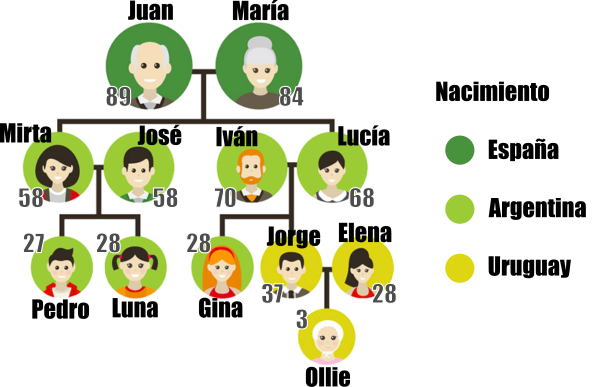
\includegraphics[height=5cm]{familia.png}
	%\end{center}
	

\end{enumerate}

\end{document}